
\documentclass[11pt,a4paper]{article}
\usepackage[utf8]{inputenc}
\usepackage[T1]{fontenc}
\usepackage[spanish,es-nodecimaldot]{babel}
\usepackage[a4paper,left=1.7cm,right=1.7cm,top=20mm,bottom=20mm]{geometry}
\usepackage{amsmath,amssymb,amsfonts,mathtools,bm}
\usepackage{braket}
\usepackage{graphicx}
\usepackage{float}
\usepackage{booktabs}
\usepackage{enumitem}
\usepackage{xcolor}
\usepackage{lmodern,microtype}
\usepackage{fancyhdr}
\usepackage{titlesec}
\usepackage[colorlinks=true,linkcolor=black,urlcolor=black,citecolor=black]{hyperref}
\numberwithin{equation}{section}
\renewcommand{\boxed}[1]{#1}
\setlength{\parindent}{0pt}
\setlength{\parskip}{5pt}
\newcommand{\dd}{\,\mathrm d}
\newcommand{\ii}{\mathrm i}
\newcommand{\e}{\mathrm e}
\newcommand{\hb}{\hbar}
\newcommand{\R}{\mathbb R}
\newcommand{\C}{\mathbb C}
\newcommand{\id}{\mathbb I}

\pagestyle{fancy}
\setlength{\headheight}{14pt}
\fancyhf{}
\fancyhead[L]{\textit{Tarea 3}}
\fancyhead[R]{Física VII: Introducción a la Mecánica Cuántica}
\begin{document}
\begin{titlepage}
\centering
\vspace*{1.8cm}

\includegraphics[width=.22\textwidth]{UdeC_escudo.png}
\vspace{1.1cm}

{\Huge\bfseries Tarea 3\par}
\vspace{.4cm}
{\Huge\bfseries Física VII: Introducción a la Mecánica Cuántica\par}
\vspace{1.5cm}
{\Large José Ignacio Rosas Sepúlveda\par}
\vspace{.8cm}
{\Large Solución\par}
\vfill
\thispagestyle{empty}
\end{titlepage}
\tableofcontents
\newpage
\section*{Enunciado}
\addcontentsline{toc}{section}{Enunciado}
\begin{enumerate}[label=\arabic*.-]
\item Considere una partícula dentro de una caja unidimensional de ancho $a$, con paredes infinitas en $x=0$ y $x=a$. En $t=0$,
\begin{equation}
\psi(x,0)=\begin{cases}
N\left[1-\cos\left(\dfrac{2\pi x}{a}\right)\right],&0\le x\le a,\\
0,&x<0\ \text{o}\ x>a,
\end{cases}
\end{equation}
donde $N$ es real y positivo.
\begin{enumerate}[label=\alph*)]
\item Encuentre $N$ para que $\psi(x,0)$ esté normalizada.
\item Calcule $\langle X(0)\rangle$ y $\Delta X(0)$.
\item Calcule la probabilidad de encontrar la partícula en $x\in[\langle X\rangle-\Delta X/2,\langle X\rangle+\Delta X/2]$.
\item Encuentre la distribución $\operatorname{prob}(E_n)$ asociada a los valores permitidos de energía.
\item Compruebe que las probabilidades del inciso anterior suman uno.
\item Encuentre $\langle E\rangle$ y $\Delta E$.
\item Calcule la probabilidad de obtener $E_n>\langle E\rangle$.
\item Encuentre $\psi(x,t)$.
\item Grafique $a|\psi(x,t)|^2$ como función de $x/a$ para distintos valores de $\tau=E_1t/\hbar$.
\end{enumerate}

\item Una partícula está inicialmente en el estado fundamental de una caja de ancho $a$. El ancho se aumenta súbitamente y de manera simétrica de $a$ a $2a$, sin modificar instantáneamente la función de onda. El estado inicial queda centrado en la nueva caja:
\begin{equation}
\psi(x)=\begin{cases}
\sqrt{\dfrac{2}{a}}\sin\left[\dfrac{\pi(x-a/2)}{a}\right],&a/2\le x\le 3a/2,\\
0,&x<a/2\ \text{o}\ x>3a/2.
\end{cases}
\end{equation}
\begin{enumerate}[label=\alph*)]
\item Encuentre la nueva distribución de probabilidad asociada a los niveles de energía de la caja de ancho $2a$.
\item Encuentre $\langle E\rangle$.
\item Calcule la probabilidad de obtener una energía mayor que el valor promedio anterior.
\end{enumerate}
\end{enumerate}
En lo posible, comente sus resultados.


\section{Problema 1}
Seguimos el procedimiento de la clase: primero normalizamos $\psi(x,0)$, luego la proyectamos sobre la base de funciones propias del pozo infinito y, finalmente, hacemos evolucionar cada componente con su fase $e^{-iE_nt/\hbar}$.

Dentro de $0<x<a$,
\begin{equation}
\psi(x,0)=N\left[1-\cos\left(\frac{2\pi x}{a}\right)\right].
\end{equation}

\subsection{Normalización, posición y dispersión}
La normalización exige
\begin{align}
1&=N^2\int_0^a\left[1-\cos\left(\frac{2\pi x}{a}\right)\right]^2\,\mathrm dx\\
&=N^2\left[a-2\int_0^a\cos\left(\frac{2\pi x}{a}\right)\mathrm dx
+\int_0^a\cos^2\left(\frac{2\pi x}{a}\right)\mathrm dx\right]\\
&=N^2\left(a+\frac a2\right)=N^2\frac{3a}{2}.
\end{align}
Equivalentemente, con $y=x/a$,
\begin{equation}
1=N^2a\int_0^1(1-\cos2\pi y)^2\dd y=N^2a\frac32,
\end{equation}
de donde
\begin{equation}
\boxed{N=\sqrt{\frac{2}{3a}}.}
\end{equation}
Por simetría respecto de $x=a/2$,
\begin{equation}
\boxed{\langle X\rangle=\frac a2.}
\end{equation}
Además,
\begin{equation}
\langle X^2\rangle=a^2\left(\frac13-\frac{5}{8\pi^2}\right),
\end{equation}
y por tanto
\begin{equation}
\boxed{\Delta X=a\sqrt{\frac1{12}-\frac{5}{8\pi^2}}
\simeq0.141448\,a.}
\end{equation}
La región solicitada es $x/a\in[0.429276,0.570724]$. Integrando la densidad en ese intervalo,
\begin{equation}
\boxed{P\simeq0.365083.}
\end{equation}

\subsection{Distribución de energía}
Los estados propios son
\begin{equation}
\varphi_n(x)=\sqrt{\frac2a}\sin\left(\frac{n\pi x}{a}\right),\qquad
E_n=n^2E_1,\qquad E_1=\frac{\pi^2\hb^2}{2ma^2}.
\end{equation}
Las amplitudes son
\begin{align}
c_n&=\int_0^a\varphi_n^*(x)\psi(x,0)\,\mathrm dx\\
&=\sqrt{\frac{4}{3a^2}}\int_0^a\sin\left(\frac{n\pi x}{a}\right)
\left[1-\cos\left(\frac{2\pi x}{a}\right)\right]\,\mathrm dx.
\end{align}
Usando $\sin A\cos B=[\sin(A+B)+\sin(A-B)]/2$ y evaluando las integrales seno en $[0,a]$, se obtiene cero para $n$ par y, para $n$ impar,
\begin{equation}
c_n=\begin{cases}
\displaystyle \frac{16\sqrt3}{3\pi n(4-n^2)},& n\ \text{impar},\\[6pt]
0,& n\ \text{par}.
\end{cases}
\end{equation}
Así,
\begin{equation}
\boxed{P(E_n)=|c_n|^2=\begin{cases}
\displaystyle\frac{256}{3\pi^2n^2(n^2-4)^2},&n\ \text{impar},\\[5pt]0,&n\ \text{par}.
\end{cases}}
\end{equation}
Como $\{\varphi_n\}$ es una base ortonormal completa, la normalización del estado implica
\begin{equation}
\sum_{n=1}^{\infty}|c_n|^2=\langle\psi(0)|\psi(0)\rangle=1.
\end{equation}
Esta es la misma comprobación de completitud usada en la clase y sirve como control independiente de la distribución obtenida.

Para los momentos de energía es más eficiente usar el operador. Como
\begin{equation}
H=-\frac{\hb^2}{2m}\frac{\dd^2}{\dd x^2},
\end{equation}
se obtiene
\begin{equation}
\boxed{\langle H\rangle=\frac43E_1,\qquad
\langle H^2\rangle=\frac{16}{3}E_1^2,
\qquad \Delta E=\frac{4\sqrt2}{3}E_1.}
\end{equation}
La condición $E_n>\langle H\rangle$ equivale a $n\ge2$; como los $n$ pares no contribuyen, el primer término es $n=3$. Por tanto
\begin{equation}
\boxed{P(E_n>\langle H\rangle)=1-|c_1|^2=1-\frac{256}{27\pi^2}\simeq0.03925.}
\end{equation}

La evolución temporal es
\begin{equation}
\boxed{\psi(x,t)=\sum_{\substack{n=1\\ n\,{\rm impar}}}^{\infty}
c_n\varphi_n(x)\e^{-\ii n^2E_1t/\hb}.}
\end{equation}
\begin{figure}[H]\centering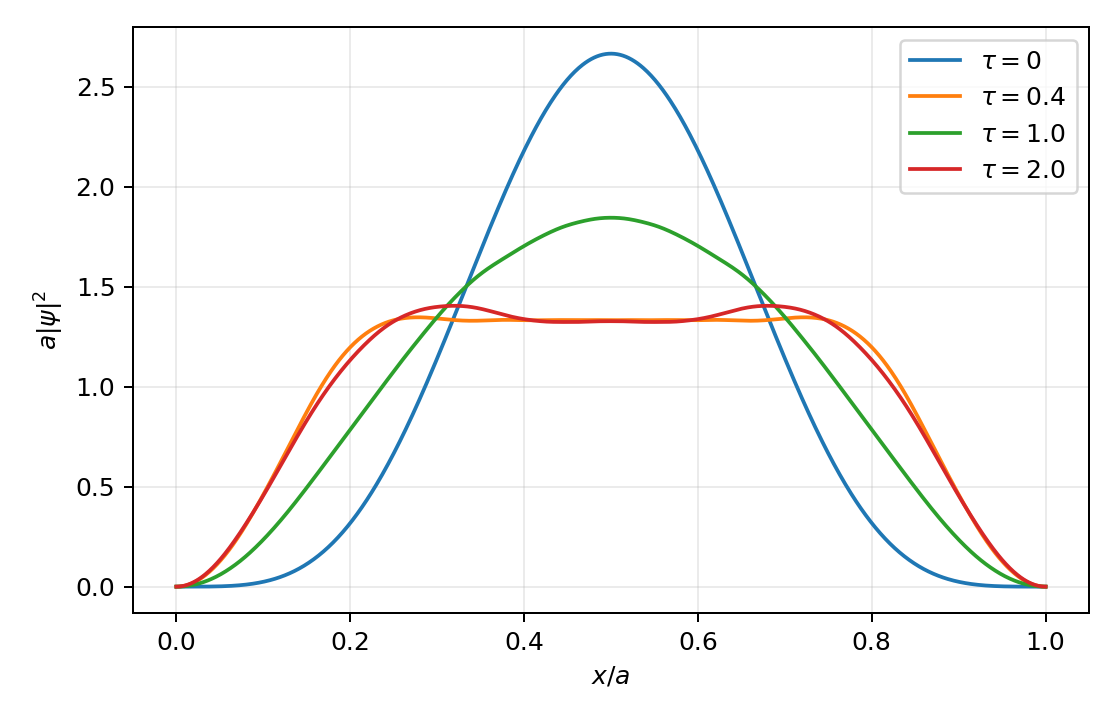
\includegraphics[width=.72\textwidth]{figures/densidad_tiempo.png}\caption{Evolución de la densidad; $\tau=E_1t/\hb$.}\end{figure}

\section{Problema 2}
Luego de expandir la caja a ancho $2a$, los nuevos estados son
\begin{equation}
\Phi_n(x)=\frac1{\sqrt a}\sin\left(\frac{n\pi x}{2a}\right),\qquad
\mathcal E_n=\frac{n^2}{4}E_1.
\end{equation}
En la aproximación súbita la función de onda no alcanza a cambiar durante la modificación de las paredes. Por eso, inmediatamente después del cambio, la misma función debe expandirse en la nueva base $\{\Phi_n\}$. Sus componentes son
\begin{equation}
d_n=\sqrt2\int_{1/2}^{3/2}\sin\left(\frac{n\pi y}{2}\right)
\sin\left[\pi\left(y-\frac12\right)\right]\dd y.
\end{equation}
Para $n\neq2$,
\begin{equation}
\boxed{d_n=-\frac{4\sqrt2}{\pi(n^2-4)}
\left[\sin\left(\frac{n\pi}{4}\right)+\sin\left(\frac{3n\pi}{4}\right)\right],}
\end{equation}
y $d_2=0$. En particular sólo contribuyen $n$ impares. La nueva distribución es $P(\mathcal E_n)=|d_n|^2$.

El valor medio de la energía puede obtenerse con $\int|\psi'|^2$ y permanece
\begin{equation}
\boxed{\langle H\rangle=E_1.}
\end{equation}
Como $\mathcal E_n> E_1$ requiere $n>2$,
\begin{equation}
\boxed{P(\mathcal E_n>\langle H\rangle)=1-|d_1|^2
=1-\frac{64}{9\pi^2}\simeq0.27949.}
\end{equation}

\paragraph{Comentario.}
La expansión súbita cambia el Hamiltoniano, no el vector de estado instantáneamente. Por eso el antiguo estado fundamental deja de ser estacionario y pasa a ser una superposición de muchos niveles del pozo más ancho.



\end{document}
